\section{Ontology details}

\subsection{Building blocks}

The power grid ontology is aimed to give a basis for representing power grids in terms of power production, consumption and transmission. For that purpose the following classes, as listed in figure \ref{fig:classes} were designed. 

\begin{figure}[h]
\centering
\subfloat[Class hierarchy]{\label{fig:classes}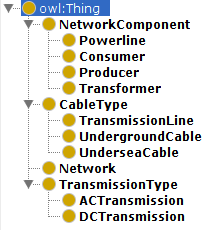
\includegraphics[width=.33\textwidth]{img/classes.png}} 
\subfloat[Object properties]{\label{fig:objProp}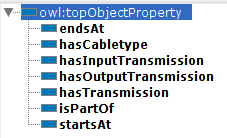
\includegraphics[width=.33\textwidth]{img/objectProperties.png}} 
\subfloat[Data properties]{\label{fig:dataProp}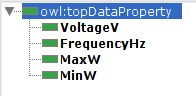
\includegraphics[width=.33\textwidth]{img/dataProperties.png}} 
\caption{Building blocks of the Power Grid ontology.}
\end{figure}

\newpage

The most basic building blocks are the \textit{NetworkComponents} which model all physical entities 
a network may consist of and are disjoint. There are \textit{Producers} adding power to the network, \textit{Consumers} drawing energy from the network, \textit{Powerlines} transporting the energy between exactly two other network entities and \textit{Transformers} managing splits, merges and changes in the transmission type of \textit{Powerlines}. \\
Those transmission types are modelled in the \textit{TransmissionType} class. This class is divided into two disjoint subclasses \textit{ACTransmission} for alternating current and \textit{DCTransmission} for direct current. \\
Each \textit{Powerline} furthermore has a \textit{CableType} indicating the layout of a power line. There are 3 disjoint alternatives: regular \textit{TransmissionLines}, \textit{UndergroundCables} and \textit{UnderseaCables}. \\
Finally every \textit{NetworkComponent} is part of a specific \textit{Network}.
The relations between the different classes written in prose above are represented in the ontology
as object properties. The domain and the range of every object property in this ontology are left blank on purpose, because they do not serve as constraint but as axioms for the reasoner. Constraints
for the object properties however are represented as subclass rules in the power grid ontology.
Every class relating to another one via an object property has a subclass rule of the type 
\begin{center}
(object property name) exactly 1 (other classes name)
\end{center}
e.g. in \textit{NetworkComponent} the following subclass rule exists:
\begin{center}
\textit{isPartOf} exactly 1 \textit{Network}
\end{center}
Apart from the \textit{isPartOf} property for \textit{NetworkComponents} other properties exist to model the relations described above. \textit{hasOutputTransmission} maps a \textit{TransmissionType} to every \textit{Producer}, \textit{hasInputTransmission} does the mapping between \textit{TransmissionType} and \textit{Consumer} and finally \textit{hasTransmission} relates a \textit{Powerline} with its \textit{TransmissionType}. Furthermore for expressing the \textit{CableType} of a \textit{Powerline} the \textit{hasCableType} entity exists. Furthermore \textit{Powerlines} need a starting- end an endpoint so \textit{startsAt} allows for \textit{Producers} or \textit{Transformers} as starting points while \textit{endsAt} respectively allows for \textit{Consumers} and \textit{Transformers} as endpoints. \\
Finally the ontology defines some data properties which quantify important measures in a power grid.
For starters every \textit{Producer} and \textit{Consumer} has a maximum power consumption expressed by the \textit{MaxW} property and a minimum power consumption expressed by the \textit{MinW} property, which are both quantified by integers. Furthermore every \textit{TransmissionType} uses a certain voltage, which is represented in the ontology by the integer property \textit{VoltageV}.
On top of that every \textit{ACTransmission} also has a certain frequency of phase shift, which in the ontology is described by the integer property \textit{FrequencyHz}. \\
Apart from the building blocks describing a power grid we also created entities forming a sample power grid. 

\subsection{A sample power grid}

All entities involved in the sample power grid can be seen in \ref{fig:entities}. The power grid uses three different types of transmission. The energy of all producers is gathered in the \textit{HighToMediumTransformer}. While the current received from the \textit{OffshoreWindFarm} via long range transmission line using the DCTransmission \textit{800kVDC} is transformed to a medium energy level ACTransmission \textit{20kV50HzAC}, the current from the \textit{BiogasPlant} already is transmitted as \textit{20kV50HzAC}. The \textit{HighToMediumTransformer} distributes energy to an \textit{IndustrialPlant}, a \textit{HousingComplex} and an employment zone having its own \textit{EmploymentZoneTransformer}. That transformer transforms the incoming current to a \textit{230V50HzAC} ACTransmission. Connected to that transformer are a \textit{Supermarket} and an
\textit{OfficeComplex}. \\
All connections between the mentioned Producers, Consumers and Transformers are Entities of the \textit{Powerline} type and named \textit{Powerline...}. Each of those power line have one of the three defined CableTypes: \textit{TransmissionLine}, \textit{UnderseaCable} or \textit{UndergroundCable}. \\
Each NetworkComponent involved is part of the \textit{SmallTownNetwork}.   

\begin{figure}
\centering
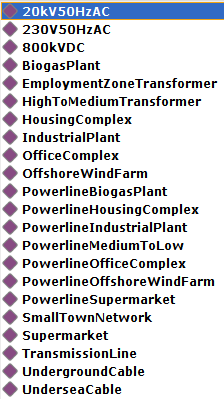
\includegraphics[width=.3\textwidth]{img/entities.png}
\caption{Entities of the sample power grid.}
\label{fig:entities}
\end{figure}

Filling in every possible data and object property involved in the construction of this sample network would have been a lot of redundant work. Therefore a set of SWRL Rules was created that allows a reasoner to induce some network properties.

\subsection{SWRL Rules}

The power grid ontology uses four rules for inducing a \textit{TransimssionType} for a \textit{NetworkComponent}, as can be seen in figure \ref{fig:swrlRules}. \\

\begin{figure}[h]
\centering
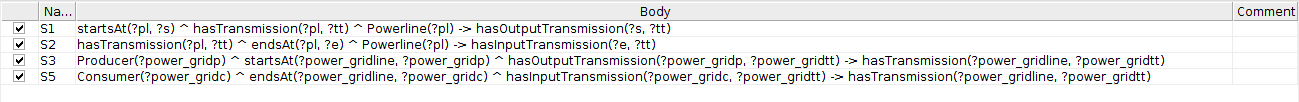
\includegraphics[width=\textwidth]{img/swrlRules.png}
\caption{SWRL Rules used in the power grid ontology.}
\label{fig:swrlRules}
\end{figure}

\newpage

The first rule says that if a \textit{Powerline} starts at $s$ and has \textit{TransmissionType} $tt$,
$s$ also has to have transmission type $tt$. \\
The second rule is the same for the endpoint:
If a \textit{Powerline} ends at $e$ and has \textit{TransmissionType} $tt$,
$e$ also has to have transmission type $tt$. \\
The third rule says if a \textit{Powerline} starts at a \textit{Producer} having \textit{TransmissionType} $tt$ it also has to have transmission type $tt$. \\
Finally the fourth rule again reflects the third one only for endpoints: 
If a \textit{Powerline} ends at a \textit{Consumer} having \textit{TransmissionType} $tt$ it also has to have transmission type $tt$.

\newpage
